\documentclass[12pt]{amsart}
% Default margins are too wide all the way around. I reset them here
\setlength{\hoffset}{-.75in}
\setlength{\textwidth}{6.5in}
\setlength{\voffset}{-.5in}
\setlength{\textheight}{9.0in}
\usepackage{amsmath}
\usepackage{amssymb}
\usepackage{amsthm}
\usepackage{pgfplots}
\usepackage{graphicx}
\pgfplotsset{compat=1.18}
\tikzset{orbit/.style={blue!70!black,thick},separatrix/.style={orange!85!black,very thick},field/.style={gray!65,-{Stealth[length=2pt,width=2pt]},line width=.3pt},equilibria/.style={black,very thick}}
\usepackage{enumerate}
\usepackage{tikz}
\usetikzlibrary{shadows,arrows,arrows.meta,shapes,positioning,calc}% Required for the Circle and Triangle arrow tips
\usepackage{setspace}
\usepackage{siunitx}
\usepackage{enumitem}
\usepackage{tcolorbox}
\usepackage{array}
\usepackage{microtype}
\usepackage{hyperref}
\usepackage{upgreek}

\theoremstyle{plain}
\newtheorem{conjecture}{Conjecture}

\theoremstyle{definition}
\newtheorem{definition}{Definition}

\theoremstyle{definition}
\newtheorem{question}{Question}

\theoremstyle{plain}
\newtheorem{theorem}{Theorem}

\newenvironment{solution}
{\begin{proof}[Solution]}
{\end{proof}}

\newcommand{\sectionrule}{%
    \vspace{0.3em}
    \hrule
    \vspace{0.8em}
}

\newcommand{\R}{\mathbb{R}}
\newcommand{\dd}{\mathop{}\!\mathrm{d}}
\newcommand{\vct}[1]{\underline{#1}}
\newcommand{\sys}[2]{\begin{aligned}#1\\#2\end{aligned}}
\newcommand{\rulehead}[1]{\vspace{2pt}\hrule\vspace{5pt}{\large\bfseries #1}\par}

\title{Dynamical Systems:\\Class September 29, 2026\\ 10. The van der Pol Oscillator}
\author{Rob Tompkins}
\date{September 29, 2026}

\begin{document}

    \maketitle
    {\large\bfseries Teams}

    Post screenshots of your work to the course Google Drive today: Link to drive folder. Include words, labels, and other short notes on your whiteboard that might make those solutions useful to you or your classmates. Name your images using the format:
    \begin{itemize}
        \item \texttt{teamXX-YY.EXT}
    \end{itemize}
    where XX is your two-digit team number (e.g. 06 if you are team 6), YY is the two digit number of image for today (e.g. 01 for the first image, 02 for the second, and so on.), and EXT is the extension for the image filetype you used.

    \par\medskip
    {\large\bfseries Team Activity}

    \section*{Problems}

    \begin{enumerate}
        \item (convince yourself of the details: van der Pol example) After a change of variables the van der Pol system is
        \[\begin{aligned}\dot x&=\mu\left(y-\frac13x^3+x\right),\\\dot y&=-\frac1\mu x.\end{aligned}\]
        Consider the case where $\mu\gg1$.
        \begin{enumerate}
            \item In this relaxation oscillation, the trajectory is moving very quickly when it jumps between the two parts of the $\dot x=0$ nullcline.

            Using the contours of the $\dot x$ equation that are provided in the plot, convince yourself that it is moving at a velocity of $c\mu$, where $c$ is between 0.1 and 2 for most of the jump.

            On the plot below, a single trajectory is shown. The $\dot x=0$ nullcline is a cubic and is drawn with a solid line. The dashed lines are the curves $y-x^3/3+x=\pm0.1$ and the dotted lines are the curves $y-x^3/3+x=\pm1.4$.
        \end{enumerate}
    \end{enumerate}
    \begin{enumerate}\item[]
        \hspace*{1.9em}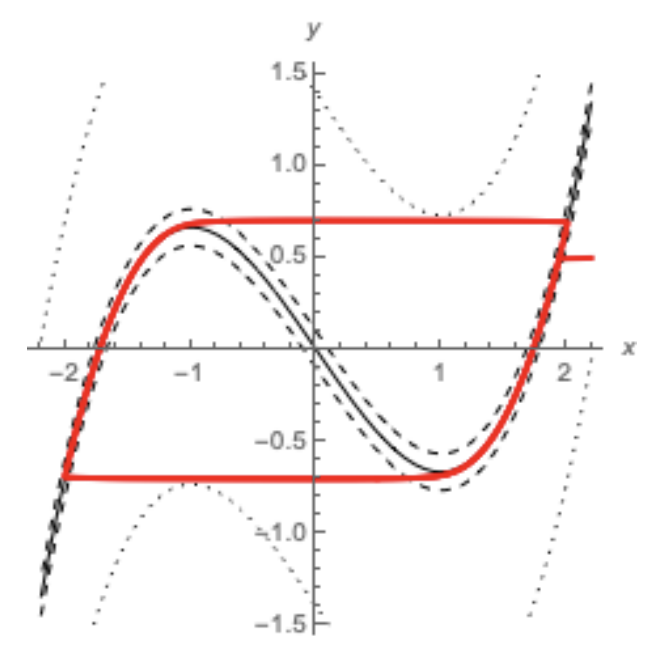
\includegraphics[width=0.53\linewidth]{figures/relaxation.png}
        \begin{enumerate}[start=2]
\item[] \emph{We sometimes say this velocity is of the order of $\mu$, or is $\mathcal O(\mu)$, because it is bounded above by a constant multiple of $\mu$.}
\item The trajectory is traversing a distance of about 3 as it jumps. Combine the approximate distance and the approximate velocity to find the $\mu$-dependence of the time that it spends jumping.
\item While moving along the nullcline, the trajectory moves about 1 unit in $x$ and a bit less than 2 units in $y$. It is basically moving along the curve $y=\frac13x^3-x$ (it is not quite on the curve, but it is close to that curve the whole time). The time it spends traversing the curve is a constant multiple of $\mu^k$ for some integer $k$.

To estimate time (just as we did for the oscillators in chapter 4), we set up an integral of the form $\int_{x_1}^{x_2}\frac{dt}{dx}\dd x$ or something like this. This integral shows us how the time depends on $\mu$. Using
\[\int_{x_1}^{x_2}\frac{dt}{dx}\dd x\]
doesn't work so well. It puts $y-(\frac13x^3-x)$ in the denominator (so a dependence on $x$ and $y$, not just $x$). What is wrong with having a dependence on $x$ and on $y$ in the integral?
\item We could try again with
\[\int_{y_1}^{y_2}\frac{dt}{dy}\dd y.\]
Argue that this leads to a problem, too, and isn't something we can integrate.
\item So actually, Steve used
\[\int_{x_1}^{x_2}\frac{dt}{dy}\frac{dy}{dx}\dd x.\]
        \end{enumerate}\end{enumerate}
    \newpage
    \begin{enumerate}\item[]
        \begin{enumerate}[start=6]
\item[] (This is an example of persisting until something works, and luckily getting something to work before we run out of options). Confirm that this expression results in something that is integrable.

Note that for $\dfrac{dy}{dx}$ we're thinking of trajectories as, to good approximation, being stuck on the nullcline, so compute this by assuming the trajectory is exactly on the nullcline.
\item Use the setup of this final integral to identify $k$. There is no need to evaluate the integral. We just want to learn the $\mu$ dependence of the time.
\item Compare the amount of time spent jumping to the amount of time spent moving along the curve. (We have the timescales of these processes, and not the exact amounts of time, so compare the timescales).
        \end{enumerate}
        Extra vocabulary / extra facts:
        \begin{itemize}
            \item A dynamical system is called \textbf{weakly nonlinear} when the system is a small perturbation away from a linear system.
            \item In its weakly nonlinear form, the van der Pol system can be written as $\ddot x+x+\epsilon\dot x(x^2-1)=0$ where $\epsilon$ is a small parameter.

            This is a small perturbation from the system $\ddot x+x=0$, which is a conservative system ($E(x,\dot x)=\frac12x^2+\frac12\dot x^2$ is conserved) and has solutions of the form $x(t)=A\cos t+B\sin t$ (for arbitrary $A$ and $B$).
            \item The presence of the $\epsilon\dot x(x^2-1)$ term changes the vector field only very slightly from the vector field in the system $\ddot x+x=0$.
            \item We can use an \textbf{energy method for approximating the location of a limit cycle} in the weakly nonlinear system. On a limit cycle, we move periodically in phase space, so $E(x,\dot x)$ will be periodic. Look at $\Delta E$ over one cycle. This will be 0 on a limit cycle, so to approximate the limit cycle, work to find a trajectory over which $\Delta E=0$.
        \end{itemize}

        \begin{solution}
        Write $F(x)=x^3/3-x$, so that $\dot x=\mu(y-F(x))$ and
        $\dot y=-x/\mu$.
        \begin{enumerate}[label=(\alph*),leftmargin=*]
            \item The contours give the horizontal speed directly:
            \[
                |\dot x|=\mu|y-F(x)|.
            \]
            On the main part of either jump, $|y-F(x)|$ is bounded away
            from zero and is of order one (roughly $0.1$ to $1.4$ in
            the figure). Thus $|\dot x|=c\mu$ with $0.1<c<2$ over most
            of the jump. Meanwhile $|\dot y|=|x|/\mu<3/\mu$, so the
            motion is almost horizontal. The upper jump goes right and
            the lower jump goes left; the stated positive quantity is
            a speed, not a signed velocity.

            \item A horizontal distance of order one traversed with
            speed of order $\mu$ takes time of order $\mu^{-1}$:
            \[
                T_{\mathrm{fast}}\sim\frac{3}{c\mu}
                =\mathcal O(\mu^{-1}).
            \]
            This estimate concerns the fast part of the jump away from
            the folds and landing points, where the speed estimate in
            part (a) applies; it is not uniform through those transition
            regions.

            \item The exact expression is
            \[
                T=\int_{x_1}^{x_2}
                \frac{1}{\mu\bigl(y(x)-F(x)\bigr)}\,\dd x.
            \]
            Here $y$ varies along the trajectory, so it cannot be treated
            as a constant. We would need the actual trajectory $y(x)$.
            Simply replacing it by $F(x)$ makes the denominator zero.
            Although the slow trajectory is close to the nullcline, it
            is not exactly on it for finite $\mu$.

            \item Similarly,
            \[
                T=\int_{y_1}^{y_2}-\frac{\mu}{x(y)}\,\dd y
            \]
            requires the relation $x=x(y)$ along the trajectory. It is
            not an explicit single-variable integrand until that relation
            is supplied. One could invert the cubic on a chosen outer
            branch as an approximation, but changing variables to $x$
            avoids that inversion.

            \item Along an outer slow branch, $y\approx F(x)$, giving
            \[
                \frac{\dd y}{\dd x}\approx F'(x)=x^2-1,
                \qquad \frac{\dd t}{\dd y}=-\frac{\mu}{x}.
            \]
            Consequently,
            \begin{align*}
                T_{\mathrm{slow}}
                &\approx-\mu\int_{x_1}^{x_2}\frac{x^2-1}{x}\,\dd x\\
                &=-\mu\left[\frac{x^2}{2}-\log|x|\right]_{x_1}^{x_2}.
            \end{align*}
            The integrand now depends only on $x$, and $x$ stays away
            from zero on each outer branch. The endpoints must follow
            the direction of motion. On the right branch $x$ decreases
            from approximately $2$ to $1$, so
            \[
                T_{\mathrm{right}}
                \approx\mu\int_1^2\left(x-\frac1x\right)\,\dd x
                =\mu\left(\frac32-\log2\right)>0.
            \]
            The left branch, traversed from $-2$ to $-1$, takes the
            same time by symmetry. This is a reduced slow-motion
            approximation, not an exact trajectory on $\dot x=0$.

            \item The integral over fixed limiting endpoints is a
            positive constant independent of $\mu$, multiplied by $\mu$.
            Hence $\boxed{k=1}$.

            \item Each slow segment takes time of order $\mu$, whereas
            the fast portion of a jump takes time of order $\mu^{-1}$.
            Their ratio therefore scales as $\mu^{-2}$, so the trajectory
            spends almost all its time on the slow branches. In
            particular, the leading period is
            \[
                \boxed{T\sim(3-2\log2)\mu\qquad(\mu\to\infty).}
            \]
        \end{enumerate}
        \end{solution}

        \setcounter{enumi}{1}
        \item (weakly nonlinear van der Pol) Let $E(x,\dot x)=\dfrac12x^2+\dfrac12\dot x^2$.
        \begin{enumerate}
            \item Find $\dfrac{dE}{dt}$ for the weakly nonlinear van der Pol oscillator, where $x+\ddot x=-\epsilon\dot x(x^2-1)$. Write $\dot E$ in terms of just $x$ and $\dot x$.
            \item We have $\Delta E=\int_0^T\frac{dE}{dt}\dd t$. The weakly nonlinear van der Pol is very close to the system $\ddot x+x=0$. Two trajectories are shown for each system in the plots below.
        \end{enumerate}\end{enumerate}
    \newpage
    \begin{enumerate}[start=2]\item[]
        \hspace*{1.9em}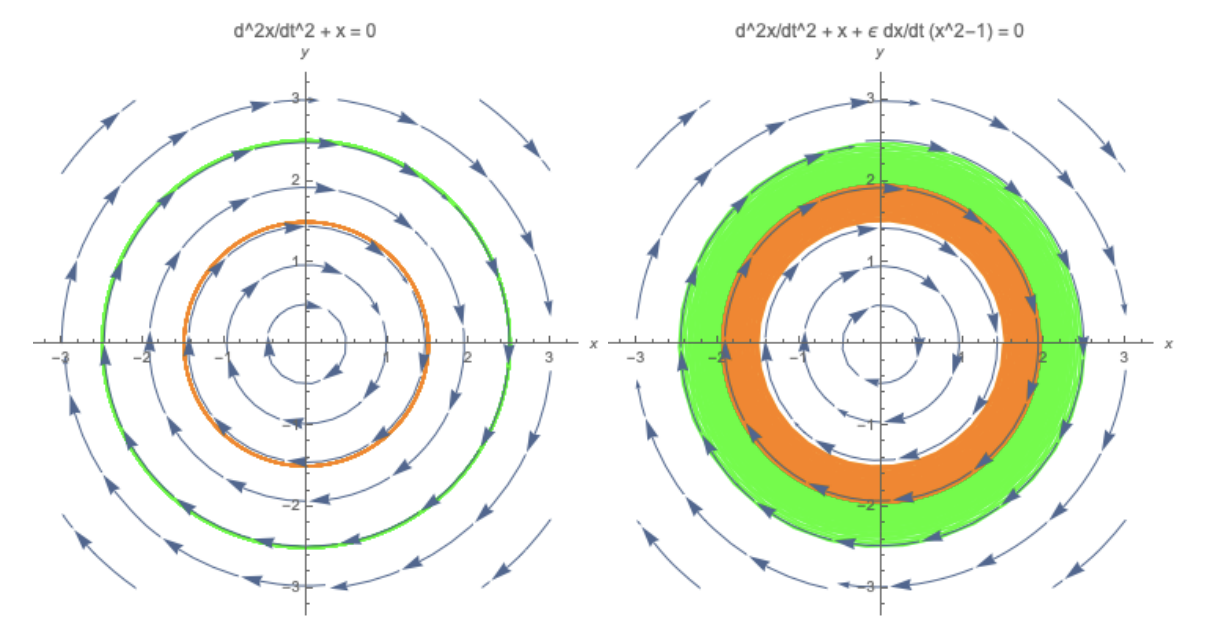
\includegraphics[width=0.94\linewidth]{figures/weakly-nonlinear.png}
        \begin{enumerate}\item[]
            In the $\ddot x+x=0$ system, the period of cycles is $T=2\pi$, and $x(t)=A\cos t$ is a solution for any $A$.

            In the weakly nonlinear van der Pol system, assume there exists a limit cycle (we know that there is one from Lienard's theorem), and that it is of the form $x(t)=A\cos t$ with period $T\approx2\pi$. We want to find the value of $A$ associated with the limit cycle.
            \begin{itemize}[itemsep=2pt,topsep=3pt]
\item Find $\dot x$ assuming $x(t)=A\cos t$.
\item Substitute $\dot x$ and $x$ into $\displaystyle\Delta E\approx-\epsilon\int_0^{2\pi}\dot x^2(x^2-1)\dd t$.
\item Using $\displaystyle\frac1{2\pi}\int_0^{2\pi}\sin^2t\dd t=\frac12$ and $\displaystyle\frac1{2\pi}\int_0^{2\pi}\cos^2t\sin^2t\dd t=\frac18$, find a value of $A$ such that $\Delta E=0$.
\item Check the $A$ you found against what is happening in the phase portrait above.
            \end{itemize}\end{enumerate}

        \begin{solution}
        \begin{enumerate}[label=(\alph*),leftmargin=*]
            \item Differentiate $E$ along a solution and use the equation
            of motion:
            \[
                \dot E=x\dot x+\dot x\ddot x
                =\dot x(x+\ddot x)
                =\boxed{-\epsilon\dot x^2(x^2-1)}.
            \]
            For $\epsilon>0$, energy increases when $|x|<1$ and decreases
            when $|x|>1$, except at points where $\dot x=0$.

            \item To leading order, $x(t)\approx A\cos t$ and
            $\dot x(t)\approx-A\sin t$. Thus
            \begin{align*}
                \Delta E
                &\approx-\epsilon\int_0^{2\pi}
                    A^2\sin^2t\,(A^2\cos^2t-1)\,\dd t\\
                &=-\epsilon\left(A^4\frac\pi4-A^2\pi\right)\\
                &=\epsilon\pi A^2\left(1-\frac{A^2}{4}\right).
            \end{align*}
            Here the supplied average identities give
            $\int_0^{2\pi}\sin^2t\,\dd t=\pi$ and
            $\int_0^{2\pi}\cos^2t\sin^2t\,\dd t=\pi/4$.
            Setting the leading energy change to zero yields
            $A=0$ or $A^2=4$. The zero solution is the equilibrium, so
            the nontrivial cycle has
            \[
                \boxed{A\approx2,\qquad T\approx2\pi.}
            \]
            For $0<A<2$, $\Delta E>0$; for $A>2$, $\Delta E<0$.
            Thus the orange inner trajectory expands and the green outer
            trajectory contracts toward the same approximately circular
            orbit $x^2+\dot x^2\approx4$, as shown in the figure.
            The sinusoid is a leading approximation for small positive
            $\epsilon$, not an exact solution of the nonlinear equation.
        \end{enumerate}
        \end{solution}

        \setcounter{enumi}{2}
        \item (Ruling out closed orbits) Let
        \[\begin{aligned}\dot x&=y,\\\dot y&=x-x^3-\mu y,\qquad\mu\geq0.\end{aligned}\]
        This system is known as the unforced Duffing oscillator. (Duffing published work on this kind of equation in 1918, and it became a popular model in the 1970s). The $\mu y$ term is a damping term.
        \begin{enumerate}
            \item This system can also be written as $\ddot x=x-x^3-\mu y$. How does this differ from the similar form that we have seen for a conservative system?
            \item Use Bendixson's criterion to show that the system has no closed orbits for $\mu>0$.
        \end{enumerate}

        \begin{solution}
        \begin{enumerate}[label=(\alph*),leftmargin=*]
            \item Since $y=\dot x$, the second-order equation is
            \[
                \ddot x+\mu\dot x-x+x^3=0.
            \]
            The conservative equation has the form $\ddot x=F(x)$,
            whereas here $-\mu\dot x$ is a velocity-dependent damping
            force. In fact, for the mechanical energy
            \[
                H(x,y)=\frac12y^2-\frac12x^2+\frac14x^4,
            \]
            differentiation gives
            \[
                \dot H=y(x-x^3-\mu y)+(-x+x^3)y=-\mu y^2.
            \]
            Thus energy is conserved when $\mu=0$ and dissipated when
            $\mu>0$ wherever $y\ne0$.

            \item For $\mathbf f(x,y)=(y,x-x^3-\mu y)$,
            \[
                \nabla\!\cdot\mathbf f
                =\frac{\partial y}{\partial x}
                 +\frac{\partial(x-x^3-\mu y)}{\partial y}
                =-\mu<0.
            \]
            The vector field is continuously differentiable on the
            simply connected plane, and its divergence has a strict,
            constant sign. Bendixson's criterion therefore rules out
            every nonconstant periodic orbit for $\boxed{\mu>0}$.
            When $\mu=0$, the divergence vanishes identically, so this
            criterion gives no exclusion.
        \end{enumerate}
        \end{solution}

        \item Find a restriction on $a$ and $b$ such that $V(x,y)=ax^2+by^2$ is a Liapunov function for
        \[\begin{aligned}\dot x&=y-x^3,\\\dot y&=-x-y^3.\end{aligned}\]
    \end{enumerate}

    \begin{solution}
        Positive definiteness of $V$ requires $a>0$ and $b>0$.
        Along a trajectory,
        \begin{align*}
            \dot V
            &=2ax(y-x^3)+2by(-x-y^3)\\
            &=2(a-b)xy-2ax^4-2by^4.
        \end{align*}
        Choosing $\boxed{a=b>0}$ cancels the mixed term and gives
        \[
            \dot V=-2a(x^4+y^4)<0\qquad\text{for }(x,y)\ne(0,0).
        \]
        Thus $V$ is a strict Lyapunov function. For example, $a=b=1$
        gives $V=x^2+y^2$.

        This equality is also necessary within the proposed quadratic
        family if $\dot V\le0$ is required in a full neighborhood of the
        origin. If $a\ne b$, choose $x=t$ and
        $y=\operatorname{sgn}(a-b)t$. Then
        \[
            \dot V=2|a-b|t^2-2(a+b)t^4>0
        \]
        for sufficiently small nonzero $t$. Hence unequal positive
        coefficients fail the Lyapunov condition. Since $V$ is radially
        unbounded and $\dot V$ is negative definite for $a=b>0$, the
        origin is globally asymptotically stable.
        \end{solution}
    \newpage
    \begin{enumerate}[start=5]
\item (trapping region for van der Pol) Consider the rectangular box shown in the figure below. The upper right and lower left corners coincide with the cubic nullcline.
\begin{center}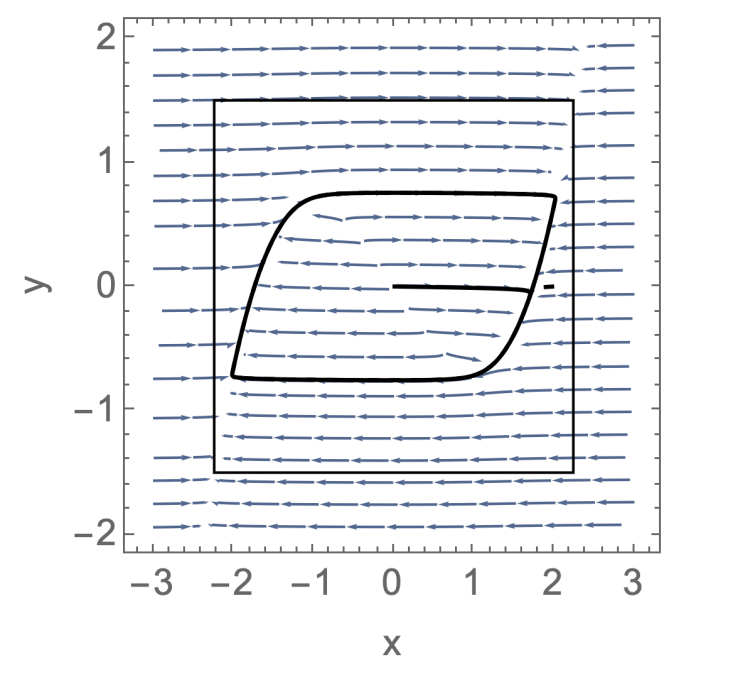
\includegraphics[width=0.65\linewidth]{figures/trapping-region.png}\end{center}
Sketch the nullclines and a vector representing the direction of the vector field in each of the four sectors created by the nullclines. Why isn't the box shown above a region that traps all trajectories? Where do trajectories escape the region?
    \end{enumerate}

    \begin{solution}
        For $\mu>0$, put $F(x)=x^3/3-x$. The nullclines are
        \[
            \dot x=0:\ y=F(x),\qquad
            \dot y=0:\ x=0.
        \]
        Above the cubic, $\dot x>0$; below it, $\dot x<0$.
        To the left of $x=0$, $\dot y>0$; to the right, $\dot y<0$.
        Thus the directions in the four regions are
        \[
        \begin{array}{c|cc}
             &y>F(x)&y<F(x)\\\hline
            x<0&\nearrow&\nwarrow\\
            x>0&\searrow&\swarrow
        \end{array}
        \]
        A schematic of the nullclines, rectangle, and these directions is:
        \begin{center}
        \begin{tikzpicture}
        \begin{axis}[
            width=.78\linewidth,height=6cm,
            xmin=-3,xmax=3,ymin=-2,ymax=2,
            axis lines=middle,xlabel={$x$},ylabel={$y$},
            xtick={-2,-1,0,1,2},ytick={-1,1},
            clip=true]
            \addplot[blue!70!black,thick,domain=-3:3,samples=160]
                {x^3/3-x};
            \addplot[orange!80!black,thick,dashed]
                coordinates {(0,-2) (0,2)};
            \draw[thick] (axis cs:-2.25,-1.546875)
                rectangle (axis cs:2.25,1.546875);
            \draw[-{Stealth},thick] (axis cs:-1.5,1)
                -- (axis cs:-1.05,1.4);
            \draw[-{Stealth},thick] (axis cs:-1.05,-.9)
                -- (axis cs:-1.5,-.5);
            \draw[-{Stealth},thick] (axis cs:1.05,1.1)
                -- (axis cs:1.5,.7);
            \draw[-{Stealth},thick] (axis cs:1.5,-1)
                -- (axis cs:1.05,-1.4);
            \draw[-{Stealth},red!75!black,very thick]
                (axis cs:-.7,1.35) -- (axis cs:-.7,1.85);
            \draw[-{Stealth},red!75!black,very thick]
                (axis cs:.7,-1.35) -- (axis cs:.7,-1.85);
        \end{axis}
        \end{tikzpicture}
        \end{center}
        The red arrows indicate outward normal components on the
        horizontal boundaries, not the full vector field.

        Write the illustrated rectangle as $[-a,a]\times[-b,b]$, with
        $b=F(a)>0$. On its top edge the outward normal is $(0,1)$, so
        \[
            \mathbf f\cdot\mathbf n=\dot y=-\frac{x}{\mu}>0
            \quad\text{when }-a<x<0.
        \]
        On the bottom edge the outward normal is $(0,-1)$, giving
        \[
            \mathbf f\cdot\mathbf n=-\dot y=\frac{x}{\mu}>0
            \quad\text{when }0<x<a.
        \]
        Hence trajectories can escape through the left half of the top
        edge and the right half of the bottom edge, so the rectangle
        is not a forward trapping region.

        The vertical edges cause no escape: on $x=a$,
        $\dot x=\mu(y-b)\le0$, and on $x=-a$,
        $\dot x=\mu(y+b)\ge0$. The field points inward or is tangent
        there. Failure of the trapping condition means that some
        trajectories leave; it does not mean that every trajectory leaves.
        \end{solution}

\end{document}